\documentclass{article}
\usepackage{amsmath, amssymb, amsthm}
\usepackage{geometry}
\usepackage{graphicx}
\usepackage{tikz}
\geometry{a4paper, margin=1in}
\usepackage{titlesec}
\usepackage{hyperref}
\setcounter{MaxMatrixCols}{20}
\newtheorem{proposition}{Proposition}
\newtheorem{definition}{Definition}
\newtheorem{theorem}{Theorem}
\newtheorem{example}{Example}

\title{Obtaining a Strongly Regular Design by Deleting a Vertex from a Rook Graph}
\author{}
\date{}

\begin{document}

\maketitle
\begin{figure}[h!]
\centering
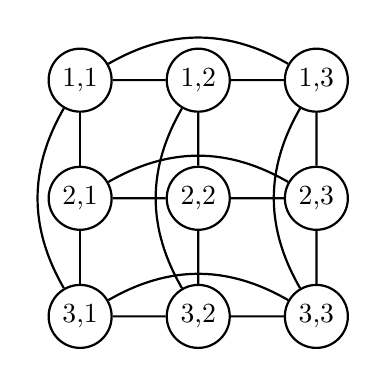
\begin{tikzpicture}[scale=1.5, every node/.style={circle, draw, inner sep=1.5pt, minimum size=0.8cm}, every path/.style={thick}]

% Define coordinates for vertices
\node (v11) at (0, 3) {1,1};
\node (v12) at (1, 3) {1,2};
\node (v13) at (2, 3) {1,3};

\node (v21) at (0, 2) {2,1};
\node (v22) at (1, 2) {2,2};
\node (v23) at (2, 2) {2,3};

\node (v31) at (0, 1) {3,1};
\node (v32) at (1, 1) {3,2};
\node (v33) at (2, 1) {3,3};

% Draw edges for rows
\foreach \i in {1,2,3} {
    \foreach \j [count=\k from 2] in {1,2} {
        \draw (v\i\j) -- (v\i\k);
    }
}

% Draw edges for columns
\foreach \j in {1,2,3} {
    \foreach \i [count=\k from 2] in {1,2} {
        \draw (v\i\j) -- (v\k\j);
    }
}

% Add curved edges to connect the corners
\draw[bend right] (v11) to (v31); % Connect (1,1) to (3,1)
\draw[bend left] (v11) to (v13); % Connect (1,1) to (1,3)
\draw[bend right] (v13) to (v33); % Connect (1,3) to (3,3)
\draw[bend left] (v31) to (v33); % Connect (3,1) to (3,3)

\draw[bend right] (v12) to (v32);
\draw[bend left] (v21) to (v23);

\end{tikzpicture}
\caption{Rook graph \( R_{3,3} \), with vertices labeled as \( (i, j) \) representing the cells of a \( 3 \times 3 \) chessboard. Edges connect vertices in the same row or column.}
\label{fig:rook-graph}
\end{figure}


\begin{abstract}
This paper explores the relationship between rook graphs and strongly regular designs. Specifically, we analyze the structural and algebraic consequences of deleting a single vertex from a rook graph. Using adjacency matrix partitioning and coherent rank, we demonstrate how this operation results in a strongly regular design, resulting in a graph with coherent rank 10.
\end{abstract}

\newpage
\section{Introduction}

Rook graphs, arising naturally from the geometry of a chessboard, provide a fascinating intersection of combinatorics and algebra. These graphs, defined by vertices corresponding to cells and edges connecting vertices in the same row or column, inherit their structure from orthogonal arrays. The inherent symmetry of these graphs leads to rich combinatorial properties.

In this paper, we investigate the effect of deleting a single vertex from a rook graph, a process that leads to the emergence of a strongly regular design. This is demonstrated using adjacency matrix partitioning and the coherent rank framework, which reflects the structural regularity of the graph.

\section{Definition of a Rook Graph}

A rook graph is defined as a graph, \(R_{n,n} = (V_R,E_R)\), where:
\begin{itemize}
    \item Vertices represent the cells of an \( n \times n \) chessboard, \(|V_R| = n^2\).
    \item Two vertices are adjacent if they lie in the same row or column on the chessboard.
\end{itemize}
An example of \(R_{3,3}\) can be seen in Figure~\ref{fig:rook-graph}. 

\section{Construction of \(R_{n,n}\)}

Alternatively, \(R_{n,n}\) can be constructed using an orthogonal array of size \( \text{OA}(2, n) \), which has the following properties:
\begin{itemize}
    \item \( \text{OA}(2, n) \) is a \( 2 \times n^2 \) matrix, where each column corresponds to a unique pair \( (x, y) \in \{1, \dots, n\} \times \{1, \dots, n\} \).
    \item For any two rows, every pair of entries appears exactly once in the same column.
\end{itemize}

We can visualise it as such:
$$
\text{OA}(2, n) = \begin{bmatrix}
    1 & 1 & \cdots & 1 & 2 & 2 & \cdots & 2 & \cdots & n & n & \cdots & n \\
    1 & 2 & \cdots & n & 1 & 2 & \cdots & n & \cdots & 1 & 2 & \cdots & n \\
\end{bmatrix}
$$

\paragraph{}
Given \( \text{OA}(2, n) \), we define the \textbf{Orthogonal Array graph} as follows:

\begin{definition}
    The Orthogonal Array graph, \(G_{OA} = (V,E)\), is constructed by OA\((2,n)\) by the following:
    \begin{itemize}
        \item Each vertex \( v_i \) corresponds to the \( i \)-th column of the orthogonal array, so \( |V| = n^2 \).
        \item Two vertices \( v_i \) and \( v_j \) are adjacent if they share the same value in any row of the array.
    \end{itemize}
\end{definition}

\paragraph{}
For \( n = 3 \), the orthogonal array \( \text{OA}(2, 3) \) is:
\[
\begin{bmatrix}
1 & 1 & 1 & 2 & 2 & 2 & 3 & 3 & 3 \\
1 & 2 & 3 & 1 & 2 & 3 & 1 & 2 & 3
\end{bmatrix}.
\]


The Orthogonal Array graph of OA\((2, 3)\) would have $9$ vertices in total, with each vertex being adjacent to 4 other vertices.
(i.e. $\begin{pmatrix}
    1\\1
\end{pmatrix}$ is adjacent to $\begin{pmatrix}
    1\\2
\end{pmatrix}$, $\begin{pmatrix}
    1\\3
\end{pmatrix}$, $\begin{pmatrix}
    2\\1
\end{pmatrix}$ and $\begin{pmatrix}
    3\\1
\end{pmatrix}$)

It can be observed that this construction of \(G\) is isomorphic to Rook graph \(R_{3,3}\), and we can generalise it to \(R_{n,n}\) as well.


\begin{theorem}
    A block graph construction of OA\((2,n)\) is isomorphic to \(R_{n,n}\).
\end{theorem}

\begin{proof} 
We want to show that the block graph construction of OA\((2,n)\), \(G = (V,E)\), is isomorphic to the Rook graph, \(R_{n,n} = (V_R, E_R)\). \\ \\
Given 
\(
\text{OA}(2, n) = \begin{bmatrix}
    1 & 1 & \cdots & 1 & 2 & 2 & \cdots & 2 & \cdots & n & n & \cdots & n \\
    1 & 2 & \cdots & n & 1 & 2 & \cdots & n & \cdots & 1 & 2 & \cdots & n \\
\end{bmatrix},
\) \\
let $G = (V,E)$ be the block graph constructed using the steps defined above. \\

We proceed as follows:
\begin{enumerate}
    \item \textbf{Vertex Sets}: 
    Since the columns of OA\((2,n)\) spans \(\{1,2,\cdots,n\}^2\), \(|V| = n^2\). Similarly, the vertices of \(R_{n,n}\) correspond to the cells of an \(n \times n\) chessboard, so \(|V_R| = n^2\). Therefore, \(|V| = |V_R|\).

    \item \textbf{Edge Sets}: 
    In \(G\), two vertices are adjacent if their corresponding columns in OA\((2,n)\) share the same value in at least one row. This means that:
    \begin{itemize}
        \item If two vertices share the same value in the top row, they are adjacent.
        \item If two vertices share the same value in the bottom row, they are adjacent.
    \end{itemize}
    This adjacency condition matches exactly how edges are defined in \(R_{n,n}\), where two cells of the chessboard are connected if they lie in the same row or column. Thus, the adjacency relationships in \(G\) and \(R_{n,n}\) are equivalent.

    \item \textbf{Bijection}: 
    
    \begin{itemize}
        \item Let \((i,j) \in V\) represent an arbitrary column in OA\((2,n)\).
        \item Let \((r_i,c_j) \in V_R\) represent a arbitrary position on a \(n\times n\) chessboard which corresponds to the \(i\)-th row and \(j\)-th column.
    \end{itemize}
    We now define a mapping \(f: V \to V_R\) as follows:
    \begin{align*}
        f((i,j)) &= (r_i,c_j), \text{  where \( (i,j) \in V \) and \((r_i,c_j) \in V_R\). }
    \end{align*}
    
    To show that the mapping is bijective, we show the following:
    \begin{itemize}
        \item \textbf{Injectivitiy}: \\
        Assume \(f((i,j)) = f((i',j'))\). Then:
        \[
        f((i,j)) = (r_i, c_j) \quad \text{and} \quad f((i',j')) = (r_{i'}, c_{j'}).
        \]
        Since \(f((i,j)) = f((i',j'))\), it follows that:
        \[
        (r_i, c_j) = (r_{i'}, c_{j'}).
        \]
        Thus, \(r_i = r_{i'}\) and \(c_j = c_{j'}\), which implies \((i,j) = (i',j')\). 
        In other words, if two positions on the \(n\times n\) chessboard are the same, their corresponding columns in the OA\((2,n)\) must be the same. \\
        Therefore, \(f\) is injective.
    
        \item \textbf{Surjectivity}: \\
        Taking an arbitrary \((r_i,c_j) \in V_R\), we need to show that there exists a \((i,j) \in V\) such that \(f((i,j)) = (r_i,c_j)\). \\
        Note that \((r_i,c_j)\) corresponds to the position on the chessboard with row \(i\) and column \(j\). Since \(f\) maps a column to a chessboard position uniquely, the 
        Since we have shown injectivity, for each \((i,j) \in V\), there is a one-to-one \(f((i,j)) = (r_i,c_j) \in V_R\). Thus, the set of images \(\{f((i,j))\text{ } | \text{ }(i,j) \in V\} \subseteq V_R\) contains exactly \(n^2\) elements. We have also shown
        Let \((x, y) \in V_R\) be an arbitrary vertex in \(R_{n,n}\). By the construction of OA\((2, n)\), there exists a column \(c = \begin{bmatrix} x \\ y \end{bmatrix} \in V\) such that the top row contains \(x\) and the bottom row contains \(y\). Thus, \(f(c) = (x, y)\), meaning every vertex in \(V_R\) has a preimage in \(V\). \\
        Therefore, \(f\) is surjective.
    \end{itemize} 
    Thus, we have shown that the mapping $f$ is a bijection.

    \item \textbf{Adjacency Preservation}: 
    If two vertices in \(G\) are adjacent, they share the same value in the top or bottom row of OA\((2,n)\). Under the mapping \(f\), this means the corresponding vertices in \(R_{n,n}\) share the same row or column. Similarly, if two vertices in \(R_{n,n}\) are adjacent, their positions share the same row or column, which corresponds to adjacency in \(G\). Thus, \(f\) preserves adjacency.

\end{enumerate}
Therefore, since $f$ is a bijection from $V\to V_R$ such that the edges are preserved, $G\cong R_{n,n}$.
    
\end{proof}

% Since we have shown isomorphism, we will understand the rook graph using the OA(2, n) construction.

\section{Deletion of One Vertex}

Rook graphs are vertex-transitive, so removing any vertex results in an equivalent graph. For simplicity, let \( v_1 \), corresponding to the coordinate \( \begin{pmatrix} 1 \\ 1 \end{pmatrix} \), be removed. 

After removal:
\begin{itemize}
    \item The degree of the \( 2(n-1) \) vertices originally adjacent to \( v_1 \) decreases by 1.
    \item All other vertices retain their original degrees.
\end{itemize}

This operation partitions the vertices into two subsets:
\begin{enumerate}
    \item The \( 2(n-1) \) vertices adjacent to \( v_1 \), corresponding to the set:
    \begin{align*}
        \left\{ \begin{pmatrix} 1 \\ 2 \end{pmatrix}, \begin{pmatrix} 1 \\ 3 \end{pmatrix},..., \begin{pmatrix} 1 \\ n \end{pmatrix}, \begin{pmatrix} 2 \\ 1 \end{pmatrix}, \begin{pmatrix} 3 \\ 1 \end{pmatrix},..., \begin{pmatrix} n \\ 1 \end{pmatrix} \right\}
    \end{align*} \\
    We shall call this set the point set, $P$.
    \item The remaining \( (n-1)^2 \) vertices, corresponding to the set:
    \begin{align*}
        \left\{ \begin{pmatrix} 2 \\ 2 \end{pmatrix}, \begin{pmatrix} 2 \\ 3 \end{pmatrix},...,\begin{pmatrix} 2 \\ n \end{pmatrix},\begin{pmatrix} 3 \\ 2 \end{pmatrix}, \begin{pmatrix} 3 \\ 3 \end{pmatrix},...,\begin{pmatrix} 3 \\ n \end{pmatrix},...,\begin{pmatrix} n \\ 2 \end{pmatrix}, \begin{pmatrix} n \\ 3 \end{pmatrix},...,\begin{pmatrix} n \\ n \end{pmatrix} \right \}
    \end{align*} \\
    We shall call this set the block set, $B$.
\end{enumerate}

\section{Adjacency Matrix Partitioning}
By grouping the vertices corresponding to $P$ and $B$ together, we end up with a matrix decomposition:
\[
\mathbf{A} =
\begin{bmatrix}
\mathbf{A}_1 & \mathbf{C} \\
\mathbf{C}^\top & \mathbf{A}_2
\end{bmatrix},
\]
where:
\begin{itemize}
    \item \( \mathbf{A}_1 \): Adjacency matrix of the Point graph \(\Gamma_P\).
    \item \( \mathbf{A}_2 \): Adjacency matrix of the Block graph \(\Gamma_B\).
\end{itemize} 
In order to observe certain properties, we aim to show that the sub-graphs \(\Gamma_P\) and \(\Gamma_B\) have specific structures:

\begin{proposition}
    \(\Gamma_P\) is the graph of two disjoint Complete graphs of size \(n-1\).%\(K_{n-1}\) graphs.
    \end{proposition}
\begin{proof}
    The point graph \(\Gamma_P\) contains vertices which correspond to elements in the set: \\
    \begin{align*}
        P = \left\{ \begin{pmatrix} 1 \\ 2 \end{pmatrix}, \begin{pmatrix} 1 \\ 3 \end{pmatrix},..., \begin{pmatrix} 1 \\ n \end{pmatrix}, \begin{pmatrix} 2 \\ 1 \end{pmatrix}, \begin{pmatrix} 3 \\ 1 \end{pmatrix},..., \begin{pmatrix} n \\ 1 \end{pmatrix} \right\}
    \end{align*}
    Let us split the set into subsets \(L\) and \(R\):
    \begin{align*}
        L &= \left\{ \begin{pmatrix} 1 \\ 2 \end{pmatrix}, \begin{pmatrix} 1 \\ 3 \end{pmatrix},..., \begin{pmatrix} 1 \\ n \end{pmatrix}\right\} = \left \{ \begin{pmatrix} 1 \\ i \end{pmatrix} \middle| \text{ }i = 2, 3, \cdots, n\right \}, \\ \\
        R &= \left\{ \begin{pmatrix} 2 \\ 1 \end{pmatrix}, \begin{pmatrix} 3 \\ 1 \end{pmatrix},..., \begin{pmatrix} n \\ 1 \end{pmatrix} \right\} = \left \{ \begin{pmatrix} i \\ 1 \end{pmatrix} \middle| \text{ }i = 2, 3, \cdots, n\right \}
    \end{align*}
    \begin{itemize}
        \item \textbf{Show disjointness of graphs}: \\
        Let \(v_L = \begin{pmatrix} 1 \\ i \end{pmatrix}\in L\) and \(v_R = \begin{pmatrix} j \\ 1 \end{pmatrix} \in R\), such that \(i, j \in \{2,3,\cdots,n\}\). For any \(v_L\) and \(v_R\), \(i \neq 1\) and \(j \neq 1\), and thus \(v_L\) will not be adjacent to \(v_R\), showing that there are no edges between the vertex sets \(L \text{ and } R\). \\
        Since we have shown that the vertex sets \(L\) and \(R\) do not have any edges, we can conclude that the graphs from \(L\) and \(R\) are disjoint.
        \item \textbf{Show that the graphs \(\Gamma_L \text{ and } \Gamma_R\) are both \(K_{n-1}\)}:
        \begin{itemize}
            \item \(\Gamma_L\): Notice that the vertices in \(L\) are adjacent to each other as the top row are all equal to 1, \(v_L = \begin{pmatrix} 1 \\ i \end{pmatrix}\in L\). Since \(|L| = n-1\), we can conclude that a Complete graph of size \(n-1\) is formed, i.e. \(K_{n-1}\)
            \item \(\Gamma_R\): Similar to the case of \(L\), we note that the vertices in \(R\) are adjacent to each other as the bottom row are all equal to 1, \(v_R = \begin{pmatrix} j \\ 1 \end{pmatrix} \in R\). Since \(|R| = n-1\), we can conclude that another Complete graph of size \(n-1\) is formed, i.e. \(K_{n-1}\)
        \end{itemize}
    \end{itemize}
     We have shown that the sub-graphs formed by vertex sets \(L\) and \(R\) are disjoint, and that \(\Gamma_L \text{ and } \Gamma_R\) are both \(K_{n-1}\) and thus have proved the proposition above.
\end{proof}

\begin{proposition}
    \(\Gamma_B\) is the block graph construction of OA\((2,n-1)\).
\end{proposition}
\begin{proof} The Block graph \(\Gamma_B\) contains vertices which correspond to elements in the set:
\begin{align*}
    B = \left\{ \begin{pmatrix} 2 \\ 2 \end{pmatrix}, \begin{pmatrix} 2 \\ 3 \end{pmatrix},...,\begin{pmatrix} 2 \\ n \end{pmatrix},\begin{pmatrix} 3 \\ 2 \end{pmatrix}, \begin{pmatrix} 3 \\ 3 \end{pmatrix},...,\begin{pmatrix} 3 \\ n \end{pmatrix},...,\begin{pmatrix} n \\ 2 \end{pmatrix}, \begin{pmatrix} n \\ 3 \end{pmatrix},...,\begin{pmatrix} n \\ n \end{pmatrix} \right \}
\end{align*}
We can generalise this set into:
\begin{align*}
    B &= \left \{ \begin{pmatrix} i \\ j \end{pmatrix} \middle | \text{ } i = \{2,3,\cdots,n\}, j = \{2,3,\cdots,n\}\right \} \\
    & = \left \{ \begin{pmatrix} i-1 + 1 \\ j-1 + 1 \end{pmatrix} \middle | \text{ } i-1 = \{1,2,\cdots,n-1\}, j-1 = \{1,2,\cdots,n-1\}\right \} \\
    &= \left \{ \begin{pmatrix} i'+1 \\ j'+1 \end{pmatrix} \middle | \text{ } i' = \{1,2,\cdots,n-1\}, j' = \{1,2,\cdots,n-1\}\right \}
\end{align*} \\
By mapping \(\begin{pmatrix} i'+1 \\ j'+1 \end{pmatrix}\) to \(\begin{pmatrix} i' \\ j' \end{pmatrix}\) by subtracting 1 from each row, we can show that \(\Gamma_B\) is isomorphic to a block graph constructed by OA\((2,n-1)\).
\end{proof}

From this decomposition, we can tell that \(\Gamma_P\) and \(\Gamma_B\) both are type-3 graphs, corresponding to a \(\begin{bmatrix}
    3 &  \\
      & 3
\end{bmatrix}\) type structure of the original \(\mathbf{A} = A(\Gamma)\).
This design structure is akin to the Strongly regular design described by Sankey\cite{sankey_srd}, which has a type matrix:
\[
\begin{bmatrix}
    3 & 2 \\
    & 3
\end{bmatrix}
\]

\section{Exploring the Coherent Structure and SRD Properties of Sub-matrices}
To show that \(\mathbf{A}\) decomposes into the Strongly regular design of type \(\begin{bmatrix}
    3 & 2 \\
    & 3
\end{bmatrix}\), we need to verify that the equations from Sankey holds. Mainly, the equations are as follows:
\begin{definition}
    A strongly regular design is a finite incidence structure consisting of a set \(X_1\) of points, a set \(X_2\) of blocks, and an incidence relation \(F \subseteq X_1 \times X_2\), such that the following are nonnegative integer constants:
    \begin{itemize}
        \item \(S_1 :=\) number of points incident with (in) each block;
        \item \(S_2 :=\) number of blocks incident with (containing) each point;
        \item \(a_1,b_1\) := the two distinct block intersection sizes;
        \item \(a_2,b_2\) := the two distinct point join sizes, that is the number of blocks containing two given points;
        \item \(N_1\) \((P_1)\) := number of points adjacent to a point \(x\) and incident with a block \(y\), provided \(x\) is (is not) incident with \(y\);
        \item \(N_2\) \((P_2)\) := number of points containing a point \(x\) and adjacent with a block \(y\), given \(x\) is (is not) incident with \(y\);
    \end{itemize}
\end{definition}
Sankey also goes on to describe that the point graph, consisting of vertices from \(X_1\), and the block graph, consisting of vertices from \(X_2\), are strongly regular. This corresponds to the earlier propositions of \(\Gamma_P\) and \(\Gamma_B\) being type-3 graphs.\\
The only thing left is to verify the remaining piece of the puzzle, the incidence matrix \(\mathbf{C}\) as Sankey describes it.
\begin{definition}
    Let \(\mathbf{C}\) be the 0/1 incidence matrix with rows indexed by the \(n_1 := |X_1|\) points and columns indexed by the \(n_2 := |X_2|\) blocks. Then, letting \(I\) be the identity matrix and \(J\) be the all ones matrix of the appropriate dimensions, we have the following equations:
    \begin{enumerate}
        \item \(\mathbf{C}\) has row sum \(S_2\) and column sum \(S_1\);
        \item \(\mathbf{CC^T} = (S_2-b_2)I + (a_2 - b_2)\mathbf{A_1} +b_2J\);
        \item \(\mathbf{C^T C} = (S_1-b_1)I + (a_1-b_1)\mathbf{A_2}+b_1J\);
        \item \(\mathbf{CA_2} = (N_2-P_2)\mathbf{C}+P_2J\);
        \item \(\mathbf{A_1C} = (N_1-P_1)\mathbf{C}+P_1J\).
    \end{enumerate}
\end{definition}

In order to check these statements, we first have to construct the matrix \(\mathbf{C}\).

\subsection{Construction of \( \mathbf{C} \)}
We know the rows of \(\mathbf{C}\) are indexed by the set \(P\) and columns are indexed by the set \(B\). To make things simple, we first consider the top half of \(\mathbf{C}\), denoted by \(\mathbf{C_1}\) with rows indexed by the set \(L\) and columns indexed by \(B\).

\paragraph{\( \mathbf{C_1} \):}

For \( \mathbf{C_1} \), the rows are indexed by:
\begin{align*}
    L &= \left\{\begin{pmatrix} 1 \\ 2 \end{pmatrix}, \begin{pmatrix} 1 \\ 3 \end{pmatrix}, \dots, \begin{pmatrix} 1 \\ n \end{pmatrix}\right\} \\
    &= \left\{ \begin{pmatrix}1 \\ i\end{pmatrix}\middle|\text{ }i\in\{2,3,\cdots,n\}\right\},
\end{align*}

while the columns are indexed by:
\begin{align*}
    B &= \left\{\begin{pmatrix} 2 \\ 2 \end{pmatrix}, \begin{pmatrix} 2 \\ 3 \end{pmatrix}, \dots, \begin{pmatrix} 2 \\ n \end{pmatrix}, \begin{pmatrix} 3 \\ 2 \end{pmatrix}, \dots, \begin{pmatrix} n \\ n \end{pmatrix}\right\} \\
    &= \left\{\begin{pmatrix}j \\k\end{pmatrix}\middle|\text{ } j,k\in\{2,3\cdots,n\}\right\}.
\end{align*}
\begin{proposition}
    Each vertex corresponding to an element in \(L\) has exactly \( n-1 \) adjacent vertices corresponding to \(n-1\) elements in \(B\).
\end{proposition}
\begin{proof}
    We aim to show any \(v_L = \begin{pmatrix}1\\i\end{pmatrix} \in L\) is adjacent to exactly \(n-1\) \(v_B = \begin{pmatrix}j\\k\end{pmatrix} \in B\). \\
    Given \(v_L = \begin{pmatrix}1\\i\end{pmatrix}\) and \(v_B = \begin{pmatrix}j\\k\end{pmatrix}\), when \(i = k\), \(v_L\) is adjacent to \(v_B\). This is the only case where adjacency occurs as \(j\neq 1, j\in\{2,3,\cdots,n\}\). \\
    Furthermore, there are \(n-1\) edges for any \(v_L\). When we set \(i=k\), there are \(|\{2,3,\cdots,n\}|=n-1\) possible values of \(j\). \\
    Thus, for any \(v_L\) there are exactly \(n-1\) adjacent vertices \(v_B\).
\end{proof}
For instance, when we fix \(i=k=2\):
\[
\begin{pmatrix} 1 \\ 2 \end{pmatrix} \text{ is adjacent to } \begin{pmatrix} 2 \\ 2 \end{pmatrix}, \begin{pmatrix} 3 \\ 2 \end{pmatrix}, \dots, \begin{pmatrix} n \\ 2 \end{pmatrix}.
\]

This adjacency results in rows of the form:
\[
[\underbrace{1 \quad 0 \quad \cdots \quad 0}_{n-1 \text{ elements}} \quad 1 \quad 0 \quad \cdots \quad 0 \quad \cdots].
\]

When repeated for \( \begin{pmatrix} 1 \\ 3 \end{pmatrix} \) onwards, \( \mathbf{C_1} \) is composed of \( n-1 \) blocks of \( I_{n-1} \):
\[
\mathbf{C_1} = 
\begin{bmatrix}
I_{n-1} & I_{n-1} & \cdots
\end{bmatrix}.
\]

Explicitly, \( \mathbf{C_1} \) looks like:
\[
\mathbf{C_1} = 
\begin{bmatrix}
1 & 0 & \cdots & 0 & 1 & 0 & \cdots & 0 & \cdots & 1 & 0 & \cdots & 0 \\
0 & 1 & \cdots & 0 & 0 & 1 & \cdots & 0 & \cdots & 0 & 1 & \cdots & 0 \\
\vdots & \vdots & \ddots & \vdots & \vdots & \vdots & \ddots & \vdots & \cdots & \vdots & \vdots & \ddots & \vdots \\
0 & 0 & \cdots & 1 & 0 & 0 & \cdots & 1 & \cdots & 0 & 0 & \cdots & 1
\end{bmatrix}.
\]

\paragraph{\( \mathbf{C_2} \):}

For \( \mathbf{C_2} \), the rows are indexed by:
\begin{align*}
R &= \left\{\begin{pmatrix} 2 \\ 1 \end{pmatrix}, \begin{pmatrix} 3 \\ 1 \end{pmatrix}, \dots, \begin{pmatrix} n \\ 1 \end{pmatrix}\right\} \\
&= \left\{\begin{pmatrix}i \\ 1\end{pmatrix}\middle |\text{ }i\in\{2,3,\cdots,n\}\right\},
\end{align*}
while the columns are still indexed by \(B\). Following the same logic as in \(\mathbf{C_1}\), we simply switch the logic from the bottom row to the top row to show adjacency.\\

This results in each row is adjacent to \( n-1 \) vertices, with \( 1 \)'s being contiguous. For instance:
\[
\begin{pmatrix} 2 \\ 1 \end{pmatrix} \text{ is adjacent to } \begin{pmatrix} 2 \\ 2 \end{pmatrix}, \begin{pmatrix} 2 \\ 3 \end{pmatrix}, \dots, \begin{pmatrix} 2 \\ n \end{pmatrix}.
\]
This results in rows of the form:
\[
[\underbrace{1 \quad 1 \quad \cdots \quad 1}_{n-1 \text{ elements}} \quad 0 \quad 0 \quad \cdots].
\]

Explicitly, \( \mathbf{C_2} \) looks like:
\[
\mathbf{C_2} = 
\begin{bmatrix}
1 & 1 & \cdots & 1 & 0 & 0 & \cdots & 0 & \cdots & 0 & 0 & \cdots & 0 \\
0 & 0 & \cdots & 0 & 1 & 1 & \cdots & 1 & \cdots & 0 & 0 & \cdots & 0 \\
\vdots & \vdots & \ddots & \vdots & \vdots & \vdots & \ddots & \vdots & \cdots & \vdots & \vdots & \ddots & \vdots \\
0 & 0 & \cdots & 0 & 0 & 0 & \cdots & 0 & \cdots & 1 & 1 & \cdots & 1
\end{bmatrix}.
\]

\paragraph{Combined Matrix \( \mathbf{C} \):}

Putting \( \mathbf{C_1} \) and \( \mathbf{C_2} \) together, the complete matrix \( \mathbf{C} \) is:
\[
\mathbf{C} = 
\begin{bmatrix}
\mathbf{C_1} \\ 
\mathbf{C_2}
\end{bmatrix}.
\]
Explicitly:
\[
\mathbf{C} = 
\begin{bmatrix}
1 & 0 & \cdots & 0 & 1 & 0 & \cdots & 0 & \cdots & 1 & 0 & \cdots & 0 \\
0 & 1 & \cdots & 0 & 0 & 1 & \cdots & 0 & \cdots & 0 & 1 & \cdots & 0 \\
\vdots & \vdots & \ddots & \vdots & \vdots & \vdots & \ddots & \vdots & \cdots & \vdots & \vdots & \ddots & \vdots \\
0 & 0 & \cdots & 1 & 0 & 0 & \cdots & 1 & \cdots & 0 & 0 & \cdots & 1 \\ \\
1 & 1 & \cdots & 1 & 0 & 0 & \cdots & 0 & \cdots & 0 & 0 & \cdots & 0 \\
0 & 0 & \cdots & 0 & 1 & 1 & \cdots & 1 & \cdots & 0 & 0 & \cdots & 0 \\
\vdots & \vdots & \ddots & \vdots & \vdots & \vdots & \ddots & \vdots & \cdots & \vdots & \vdots & \ddots & \vdots \\
0 & 0 & \cdots & 0 & 0 & 0 & \cdots & 0 & \cdots & 1 & 1 & \cdots & 1
\end{bmatrix}.
\]

With this constructed matrix \(\mathbf{C}\), we can now identify the parameters of a strongly regular design.

\begin{enumerate}
    \item The row sum of \(\mathbf{C}\) is \(n-1\), which is equal to \(S_2\).
    \item The column sum of \(\mathbf{C}\) is 2, which is equal to \(S_1\).
\end{enumerate}

We now calculate the following matrices in order to obtain the parameters and check if the equations hold:

\begin{itemize}
    \item \(\mathbf{CC^T}\)
    \begin{align*}
        \mathbf{CC^T} &=
        \begin{bmatrix}
            (n-1)I_{n-1} & J_{n-1} \\
            J_{n-1} & (n-1)I_{n-1}
        \end{bmatrix}\\
        &= (n-2)I_{2(n-1)} + \mathbf{A_1} + J_{2(n-1)}, \text{ (which corresponds to)}\\
        &= (S_2-b_2)I + (a_2-b_2)\mathbf{A_1} + b_2J
    \end{align*}
    We can form equations to identify:
    \begin{align*}
        n -2 &= S_2 - b_2 \\
        a_2 - b_2 &= 1 \\
        b_2 &= 1 \\
        \Rightarrow a_2 &= 2 \\
        \Rightarrow n-2 &= S_2 - 1 \\
        \Rightarrow S_2 &= n-1
    \end{align*}
    So we obtain \boxed{a_2=2, b_2=1, S_2=n-1}.

    \item \(\mathbf{C^T C}\)
    \begin{align*}
        \mathbf{C^T C} &=
        \begin{bmatrix}
            I_{n-1} + J_{n-1} & I_{n-1} & \cdots & I_{n-1} \\
            I_{n-1} & I_{n-1} + J_{n-1} & \cdots & I_{n-1} \\
            \vdots & \vdots & \ddots & \vdots \\
            I_{n-1} & I_{n-1} & \cdots & I_{n-1} + J_{n-1}
        \end{bmatrix} \\
        &=
        2I_{(n-1)^2} + \mathbf{A_2}, \text{ (which corresponds to)}\\
        &= (S_1-b_1)I + (a_1-b_1)\mathbf{A_2} + b_1J
    \end{align*}
    We can form equations to identify:
    \begin{align*}
        2 &= S_1 - b_1 \\
        1 &= a_1 - b_1 \\
        0 &= b_1 \\
        \Rightarrow a_1 &= 1 \\
        \Rightarrow 2 &= S_1 
    \end{align*}
    So we obtain \boxed{a_1 = 1, b_1 = 0, S_1 = 2}.
    Note that by this point we have confirmed the values of $S_1 \text{ and }S_2$ to be the column and row sum of $\mathbf{C}$ respectively.

    \item \(\mathbf{CA_2}\)
    \begin{align*}
        \mathbf{CA_2} 
        % &= \begin{bmatrix}
        %     p
        % \end{bmatrix} \\
        &= (n-3)\mathbf{C} + J,
        \text{ (which corresponds to)}\\
        &= (N_2-P_2)\mathbf{C} + P_2J
    \end{align*}
    We can form equations to identify:
    \begin{align*}
        n-3 &= N_2 - P_2 \\
        1 &= P_2 \\
        \Rightarrow N_2 &= n-2
    \end{align*}
    So we obtain \boxed{N_2 = n-2, P_2=1}.

    \item \(\mathbf{A_1C}\)
    \begin{align*}
        \mathbf{A_1C} 
        % &= \begin{bmatrix}
        %     p
        % \end{bmatrix} \\
        &= -\mathbf{C} + J,
        \text{ (which corresponds to)}\\
        &= (N_1-P_1)\mathbf{C} + P_1J
    \end{align*}
    We can form equations to identify:
    \begin{align*}
        -1 &= N_1 - P_1 \\
        1 &= P_1 \\
        \Rightarrow N_1 &= 0
    \end{align*}
    So we obtain \boxed{N_1 = 0, P_1 = 1}.
\end{itemize}

(In progress of relating it to the equations in the cited paper \cite{sankey_srd})


\newpage
\section*{Conclusion}

The deletion of one vertex from a rook graph results in a strongly regular design with coherent rank 10. This partitioning of the adjacency matrix into structured submatrices highlights the combinatorial and algebraic regularity inherent in the graph's construction. 


\bibliographystyle{unsrt}
\bibliography{references}

\end{document}
